\documentclass[fleqn,10pt]{wlscirep}
\usepackage[utf8]{inputenc}
\usepackage[T1]{fontenc}
\usepackage{float}
\usepackage {tikz}
\usepackage {pgfplots}
\usepackage {pgfplotstable}
\usepgfplotslibrary{statistics}
\usepgfplotslibrary{colorbrewer}
\pgfplotsset{compat = 1.14, cycle list/Set1-8} 
\usetikzlibrary{pgfplots.statistics, pgfplots.colorbrewer}
\usetikzlibrary{arrows,positioning,shapes,decorations.text,mindmap,backgrounds}
\usepackage{subcaption}
\title{Identity and Search on Wikipedia}

\author[1,+]{Dániel Ficzere}
\author[1,+]{Attila Frankó}
\author[1,2,+]{Zalán Heszberger}
\author[1,2,+]{József Bíró}
\author[1,2,+,*]{András Gulyás}

\affil[1]{Budapest University of Technology and Economics, Dept. of Telecommunications and Media Informatics, Budapest, H-1117, Hungary}
\affil[2]{MTA-BME Information Systems Research Group, Eötvös Loránd Research Network (ELKH)}

\affil[*]{gulyas@tmit.bme.hu}

\affil[+]{these authors contributed equally to this work}

%\keywords{Keyword1, Keyword2, Keyword3}

\begin{abstract}
Example Abstract. Abstract must not include subheadings or citations. Example Abstract. Abstract must not include subheadings or citations. Example Abstract. Abstract must not include subheadings or citations. Example Abstract. Abstract must not include subheadings or citations. Example Abstract. Abstract must not include subheadings or citations. Example Abstract. Abstract must not include subheadings or citations. Example Abstract. Abstract must not include subheadings or citations. Example Abstract. Abstract must not include subheadings or citations.
\end{abstract}
\begin{document}

\flushbottom
\maketitle
% * <john.hammersley@gmail.com> 2015-02-09T12:07:31.197Z:
%
%  Click the title above to edit the author information and abstract
%
\thispagestyle{empty}

\noindent Please note: Abbreviations should be introduced at the first mention in the main text – no abbreviations lists. Suggested structure of main text (not enforced) is provided below.

\section*{Introduction}

The Introduction section, of referenced text\cite{Figueredo:2009dg} expands on the background of the work (some overlap with the Abstract is acceptable). The introduction should not include subheadings.

\section*{Results}

Up to three levels of \textbf{subheading} are permitted. Subheadings should not be numbered.

\subsection*{Scaffold visualization}

\begin{figure}[H]
\centering
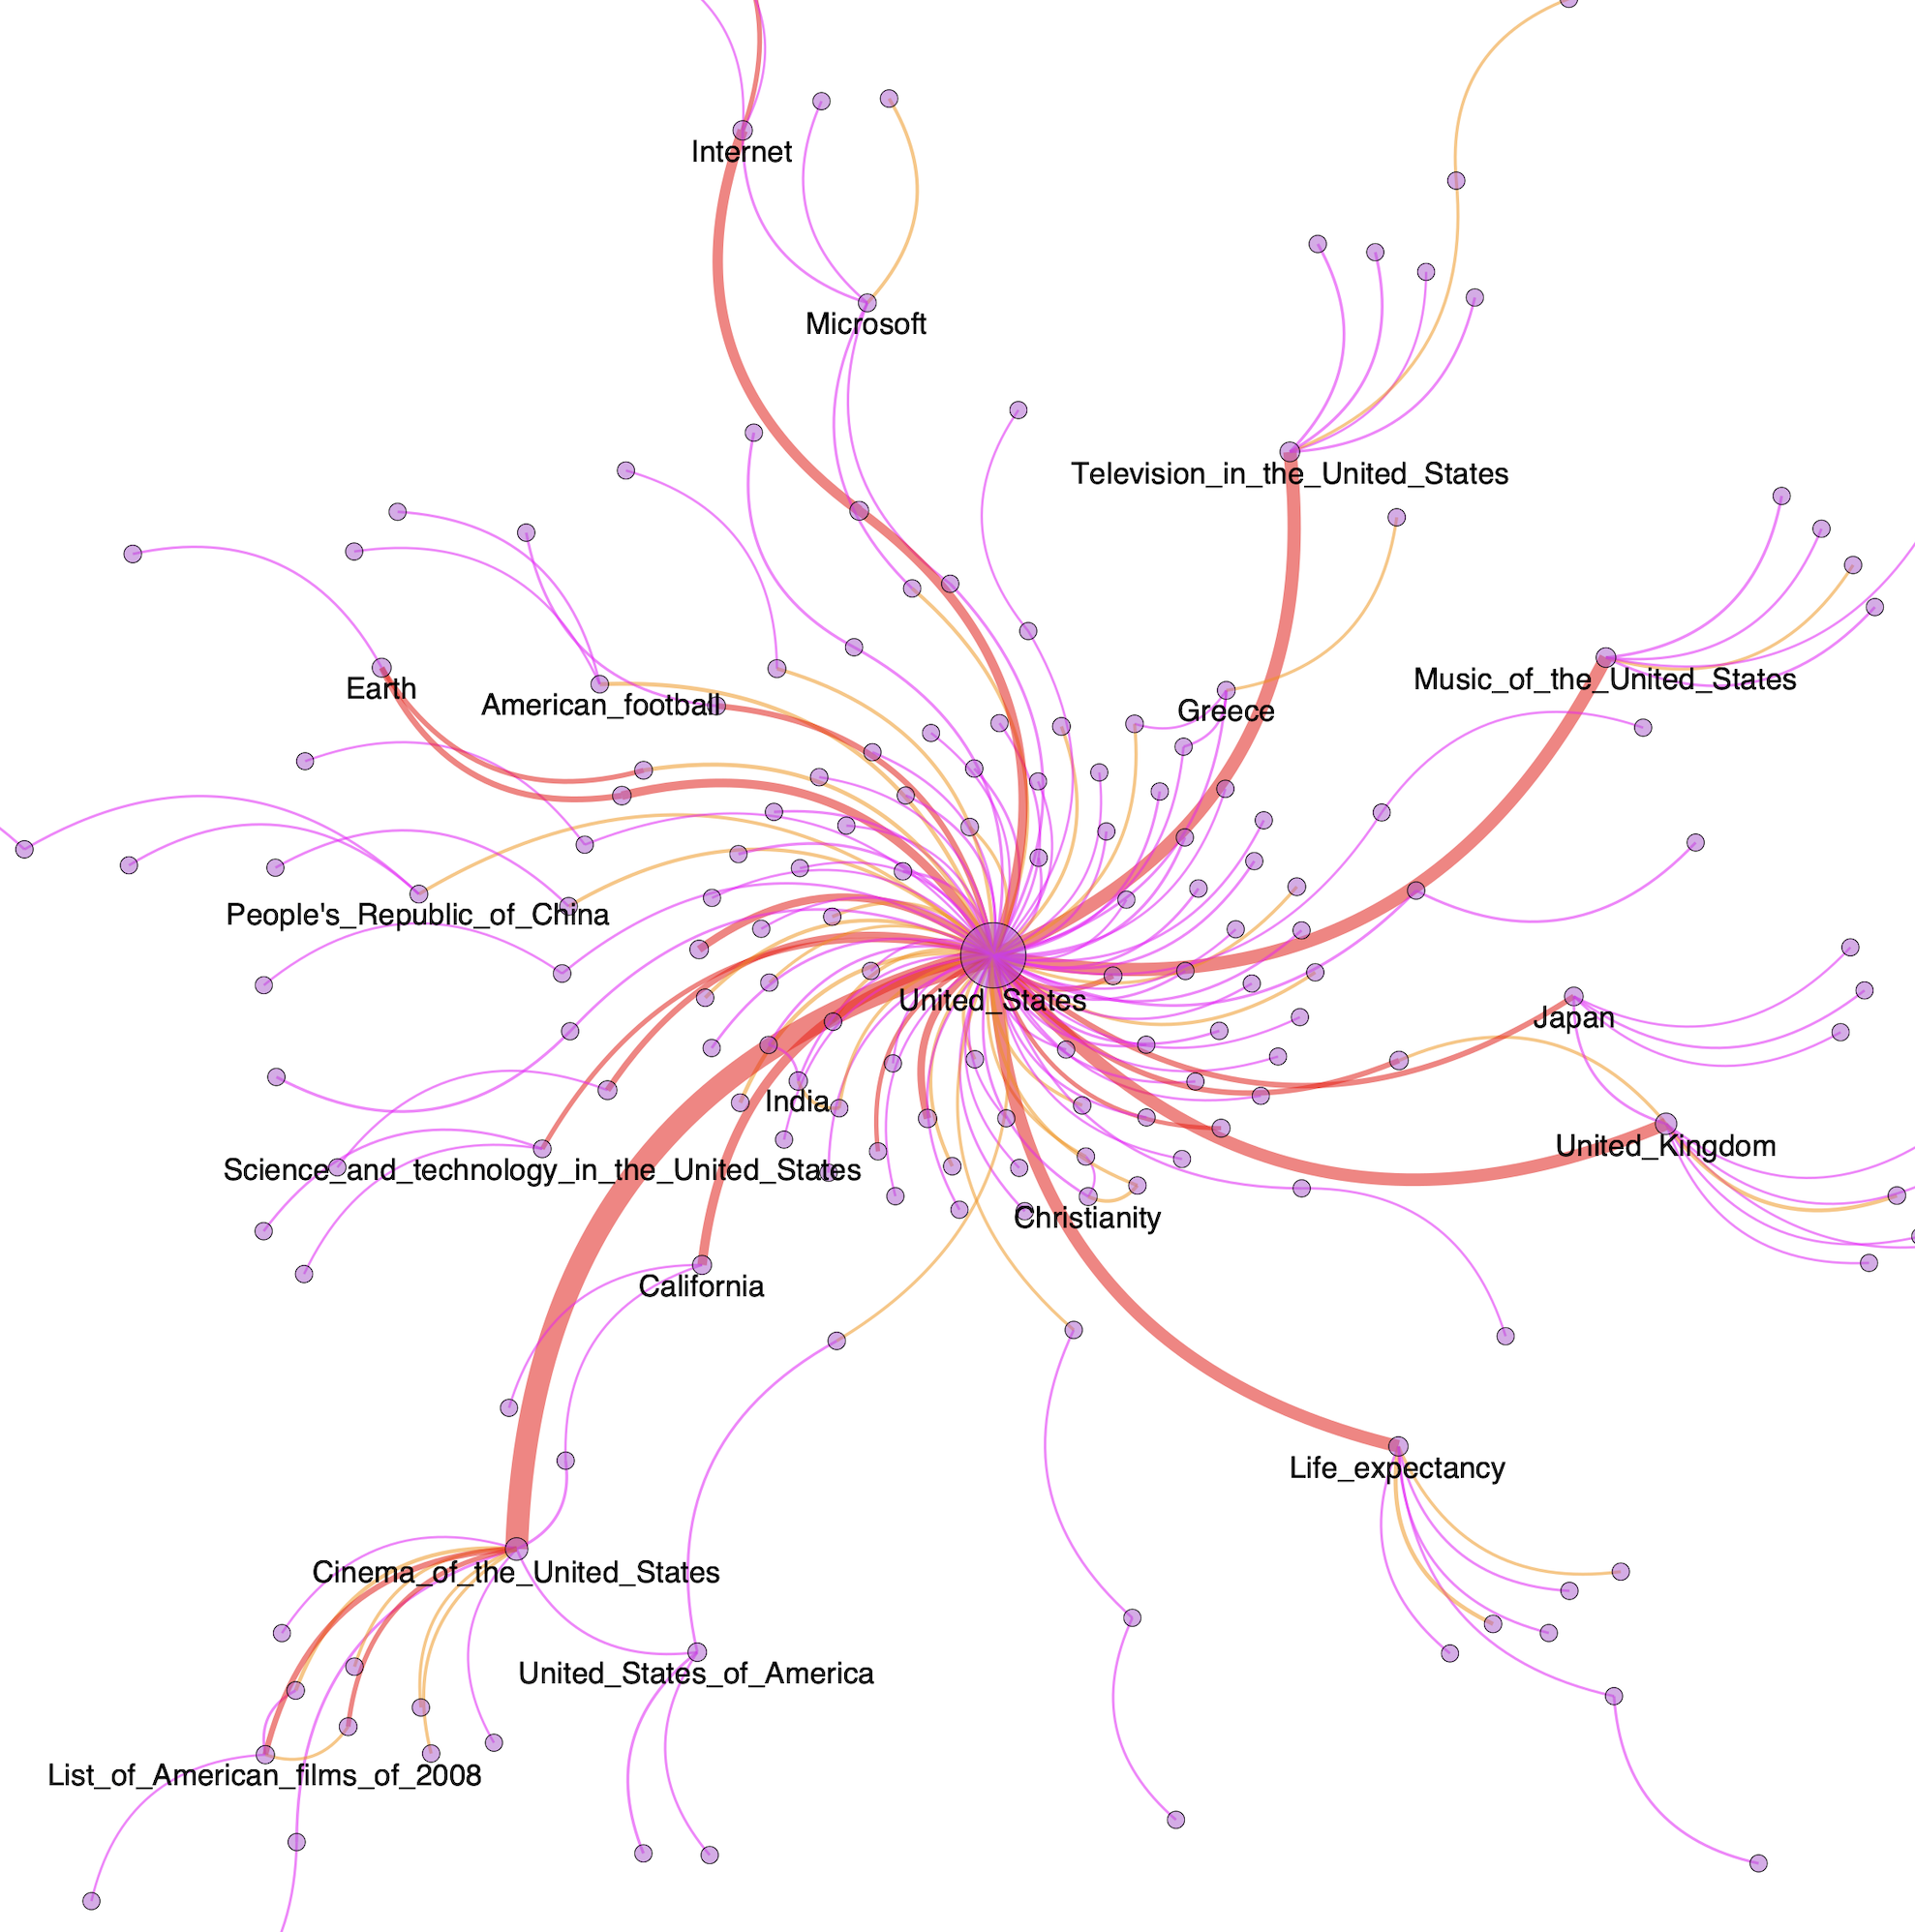
\includegraphics[width=0.7\linewidth]{figs/scaffold_vis.png}
\caption{Visualization of a user scaffold.}
\label{fig:scaffvis}
\end{figure}

\subsection*{Scaffold statistics}

\begin{figure}[H]
  \centering
    \begin{tikzpicture}
        \begin{axis}[
        xmode=log,
        ymode=log,
        height=5cm,width=8cm,
        boxplot/draw direction = y,
        x axis line style = {opacity=0},
        axis x line* = bottom,
        axis y line = left,
        enlarge y limits,
        ymin=1, ymax=60,
        xmax=70,
        cycle list={index of colormap=1 of Set1-8},
        ymajorgrids,
        xlabel = {k},
        ylabel = {Degree CDF(k)},
        ]
        \addplot+ table [x=deg, y=num, col sep=comma] {data/scaffold_degdist.txt};
        \end{axis}
    \end{tikzpicture}
    \begin{tikzpicture} 
        \begin{axis}[
        xmode=log,
        ymode=log,
        height=5cm,width=8cm,
        boxplot/draw direction = y,
        x axis line style = {opacity=0},
        axis x line* = bottom,
        axis y line = left,
        enlarge y limits,
        ymin=1, ymax=200,
        cycle list={index of colormap=1 of Set1-8},
        ymajorgrids,
        xlabel = {w},
        ylabel = {Edge weight CDF(w)},
        ]
        \addplot+ table [x=weight, y=num, col sep=comma] {data/scaffold_weightdist.txt};
        \end{axis}
    \end{tikzpicture}
  \caption{Degree and edge weight distribution in user scaffolds.}
  \label{fig:dists}
\end{figure}


\begin{figure}[H]
  \centering
    \begin{tikzpicture}
        \begin{axis}[
        height=5cm,width=4.5cm,
        boxplot/draw direction = y,
        x axis line style = {opacity=0},
        axis x line* = bottom,
        axis y line = left,
        enlarge y limits,
        ymin=0, ymax=500,
        cycle list={index of colormap=1 of Set1-8},
        ymajorgrids,
        xtick = {1,2},
        xticklabel style = {align=center, font=\small},
        xticklabels = {},
        xtick style = {draw=none}, % Hide tick line
        ylabel = {Number of nodes},
        % ytick = {20, 40}
        ]
        \addplot+[boxplot, fill, draw=black] table [y=nodes, col sep=comma] {data/scaffolds_nodes.txt};
        \end{axis}
    \end{tikzpicture}
    \begin{tikzpicture} 
        \begin{axis}[
        height=5cm,width=4.5cm,
        boxplot/draw direction = y,
        x axis line style = {opacity=0},
        axis x line* = bottom,
        axis y line = left,
        enlarge y limits,
        ymin=1.9, ymax=2.7,
        cycle list={index of colormap=1 of Set1-8},
        ymajorgrids,
        xtick = {1,2},
        xticklabel style = {align=center, font=\small},
        xticklabels = {},
        xtick style = {draw=none}, % Hide tick line
        ylabel = {Average degree},
        % ytick = {20, 40}
        ]
        \addplot+[boxplot, fill, draw=black] table [y=avgdeg, col sep=comma] {data/scaffolds_avgdeg.txt};
        \end{axis}
    \end{tikzpicture}
    \begin{tikzpicture} 
        \begin{axis}[
        height=5cm,width=4.5cm,
        boxplot/draw direction = y,
        x axis line style = {opacity=0},
        axis x line* = bottom,
        axis y line = left,
        enlarge y limits,
        ymin=2.7, ymax=5.5,
        cycle list={index of colormap=1 of Set1-8},
        ymajorgrids,
        xtick = {1,2},
        xticklabel style = {align=center, font=\small},
        xticklabels = {},
        xtick style = {draw=none}, % Hide tick line
        ylabel = {Average distance},
        % ytick = {20, 40}
        ]
        \addplot+[boxplot, fill, draw=black] table [y=avgdist, col sep=comma] {data/scaffolds_avgdist.txt};
        \end{axis}
    \end{tikzpicture}
    \begin{tikzpicture}
        \begin{axis}[
        height=5cm,width=4.5cm,
        boxplot/draw direction = y,
        x axis line style = {opacity=0},
        axis x line* = bottom,
        axis y line = left,
        enlarge y limits,
        ymin=0, ymax=0.07,
        cycle list={index of colormap=1 of Set1-8},
        ymajorgrids,
        xtick = {1,2},
        xticklabel style = {align=center, font=\small},
        xticklabels = { All scaffold pairs},
        xtick style = {draw=none}, % Hide tick line
        ylabel = {Jaccard index},
        % ytick = {20, 40}
        ]
        \addplot+[boxplot, fill, draw=black] table [y=jaccard, col sep=comma] {data/jaccards.txt};
        \end{axis}
   \end{tikzpicture}
  \caption{Statistics of user scaffolds.}
  \label{fig:bstats}
\end{figure}

\subsection*{Search dimensions}
\begin{figure}[H]
\centering
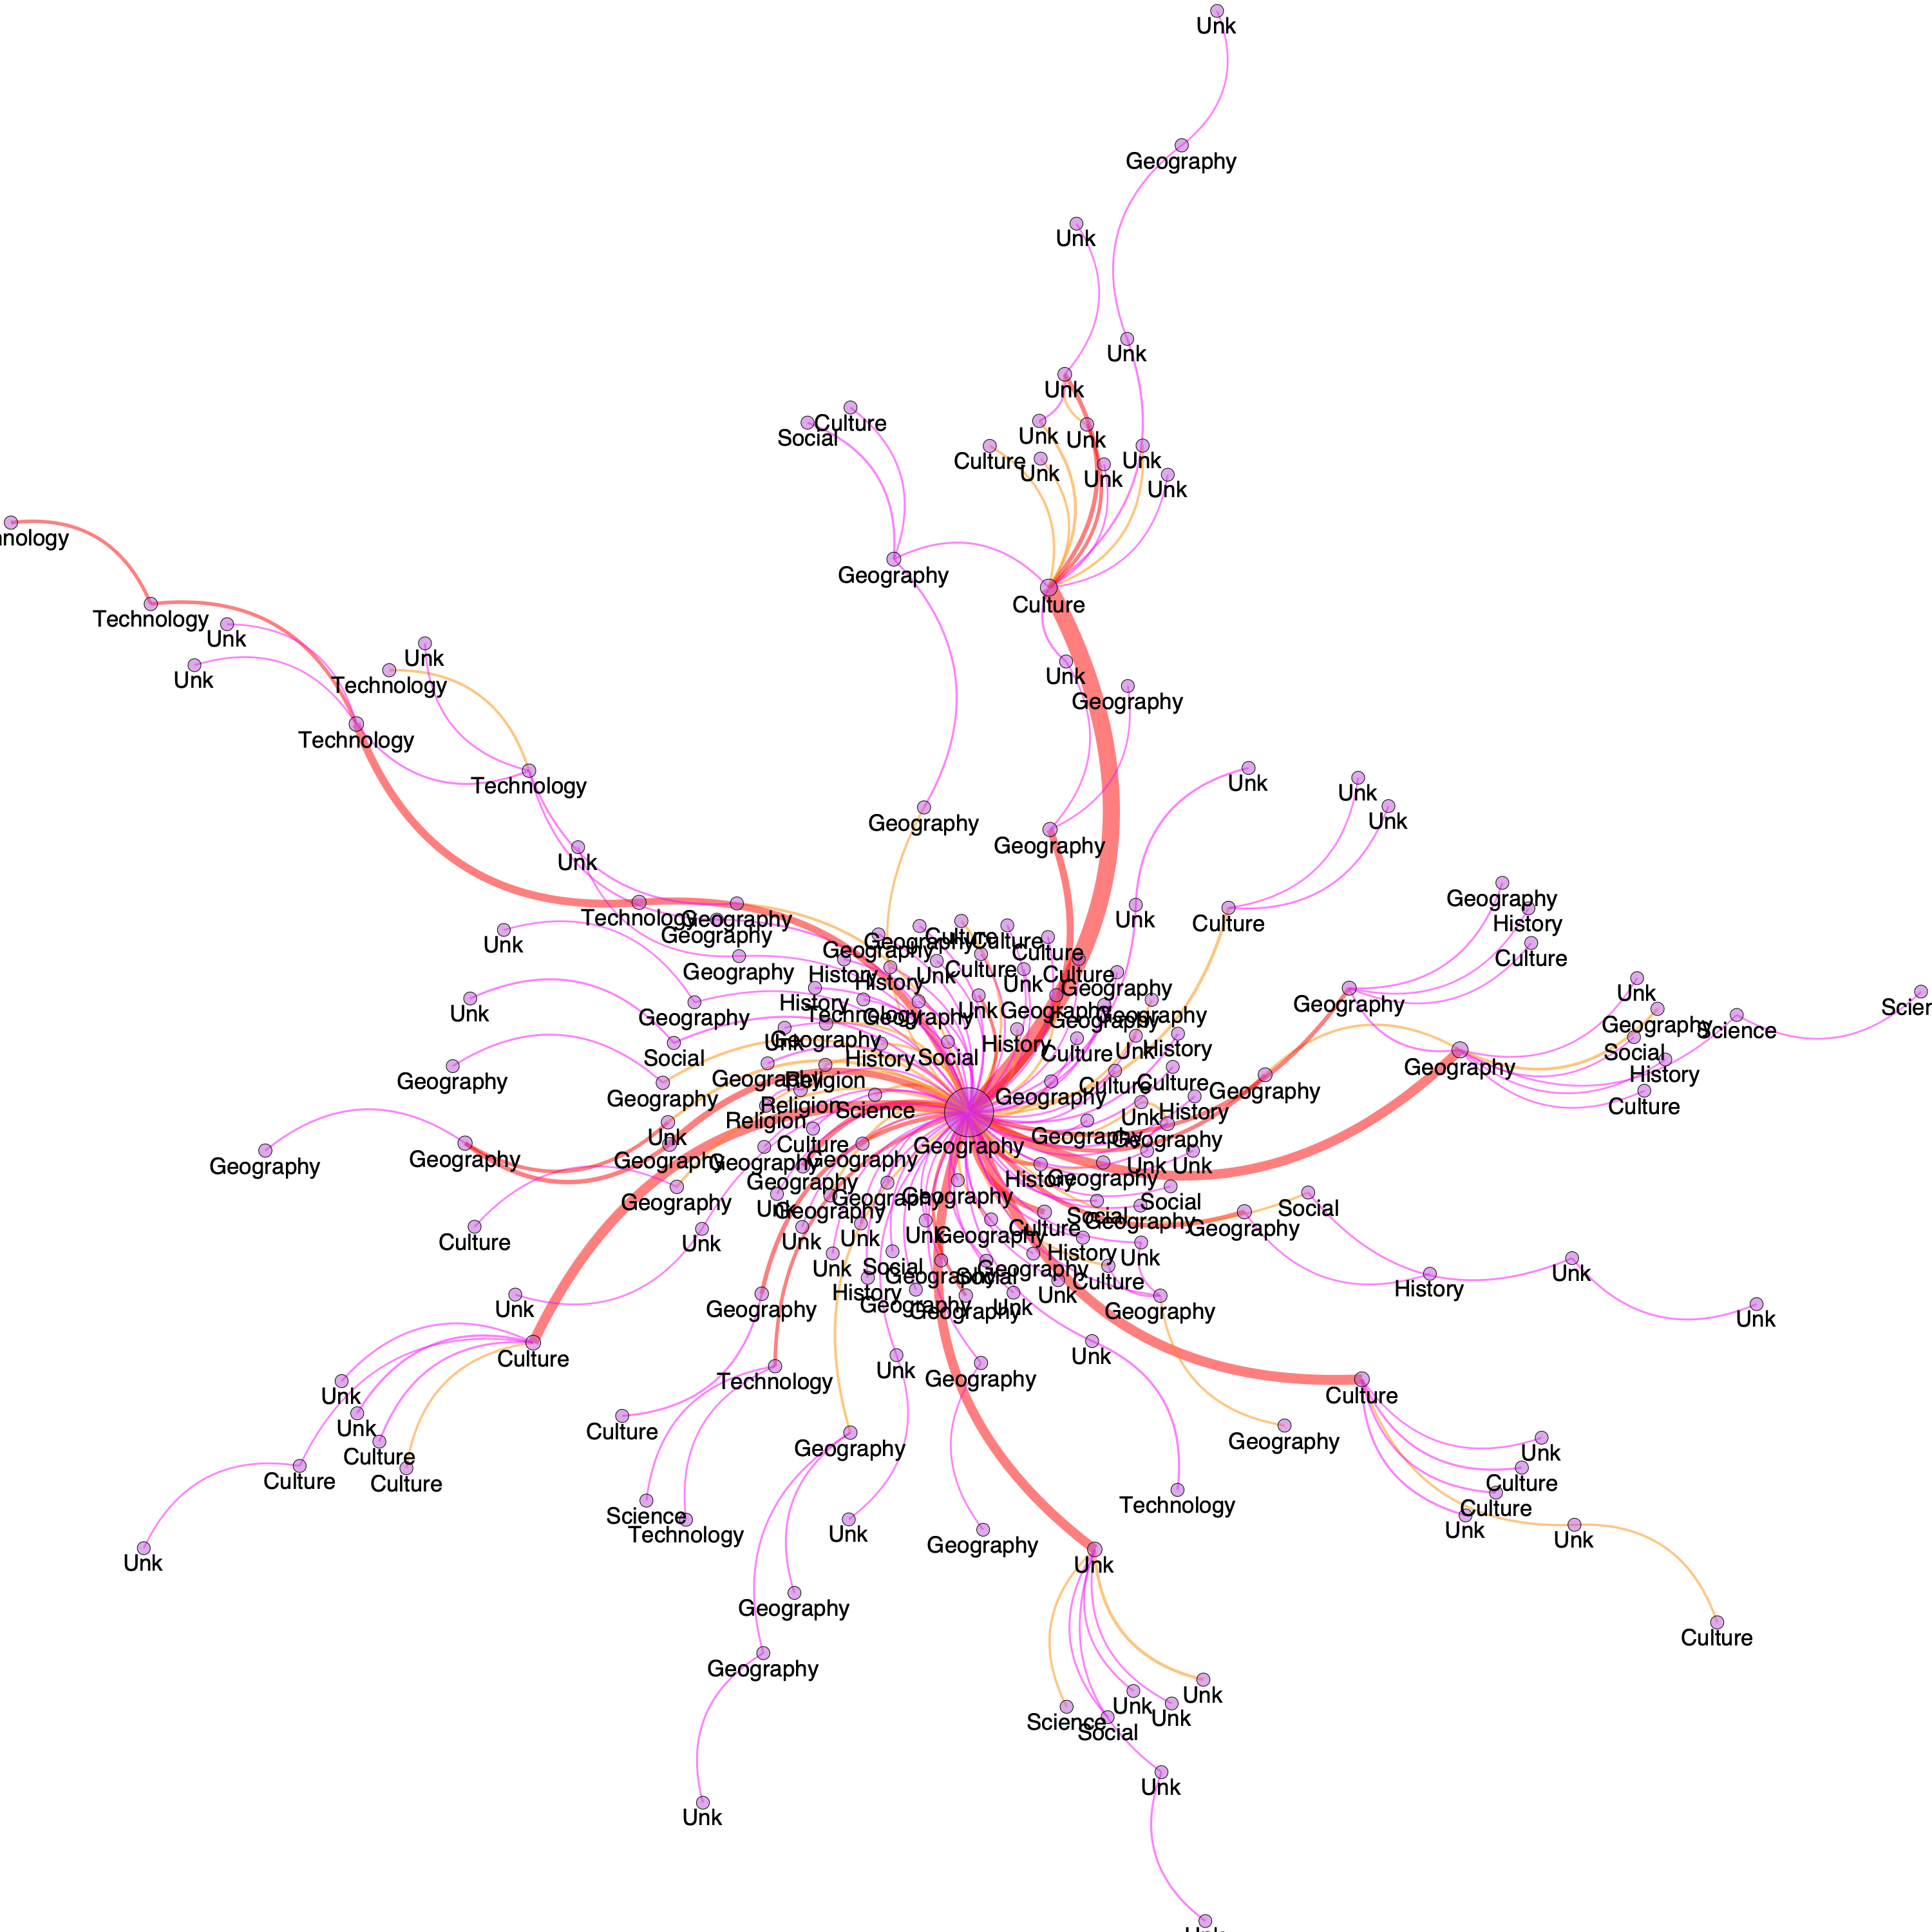
\includegraphics[width=0.32\linewidth]{figs/mysql_Mursuka_reduced_tags.png}
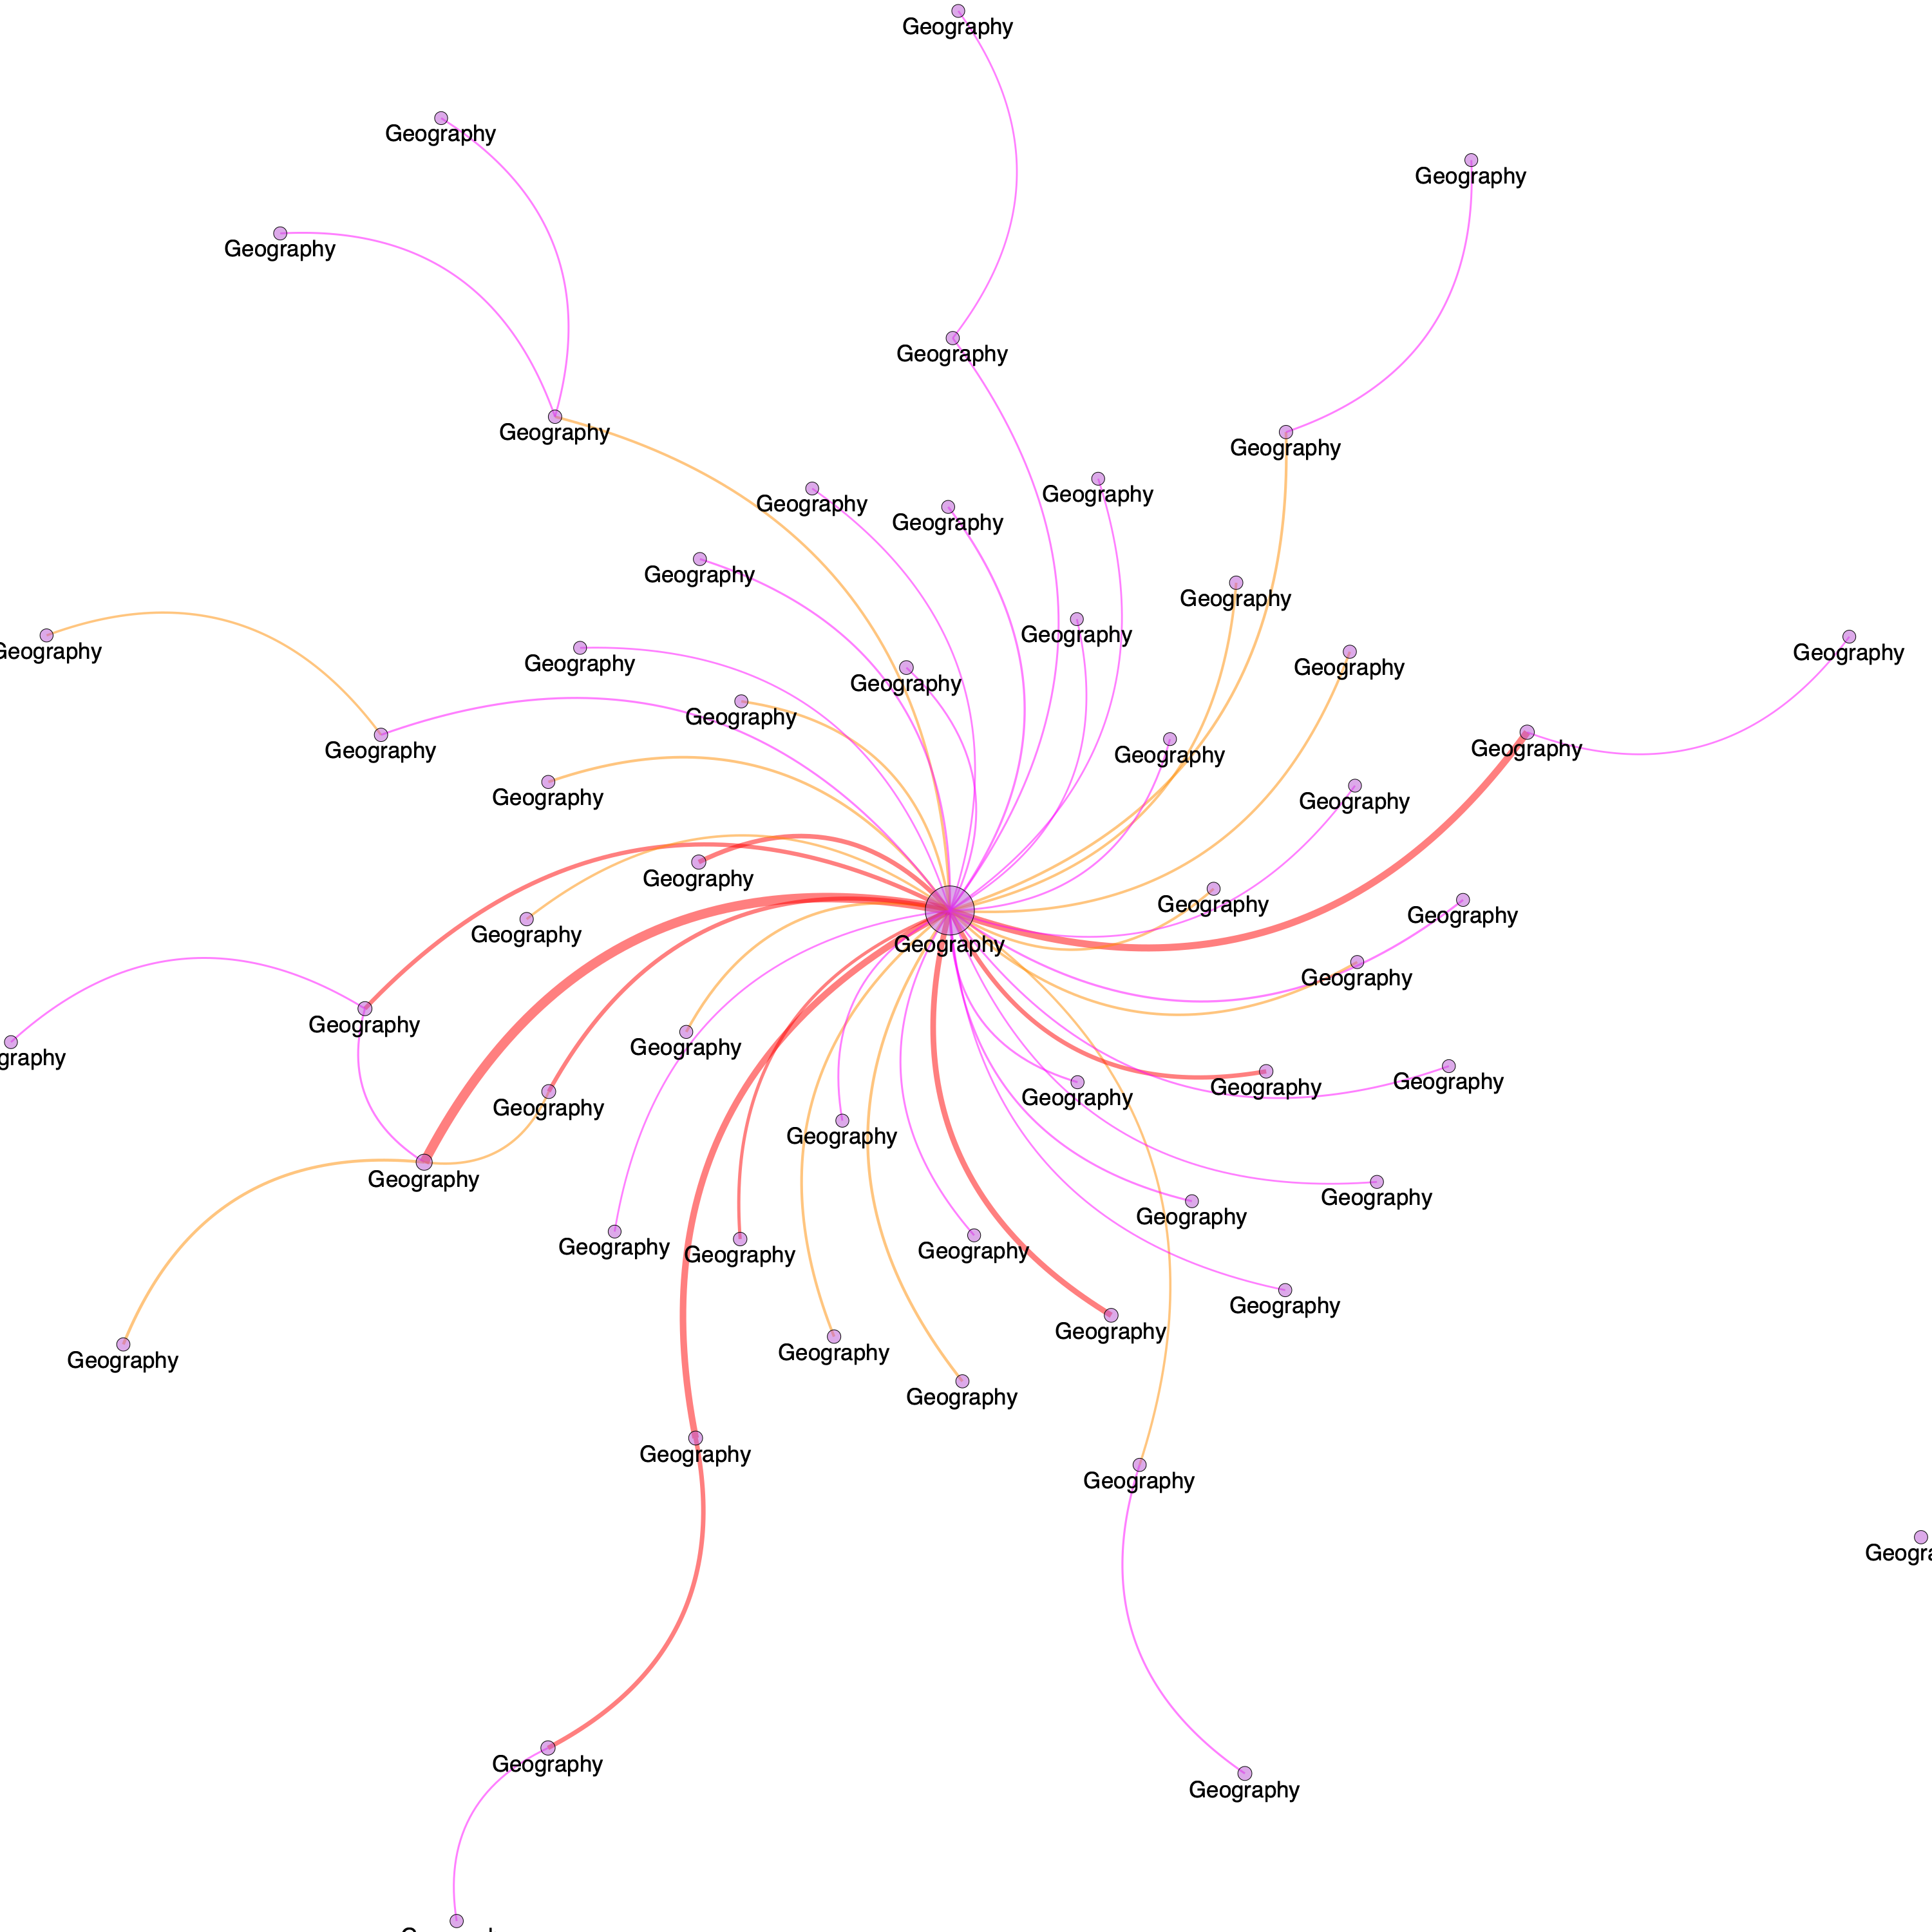
\includegraphics[width=0.32\linewidth]{figs/mysql_Mursuka_reduced_tagsub_geo.png}
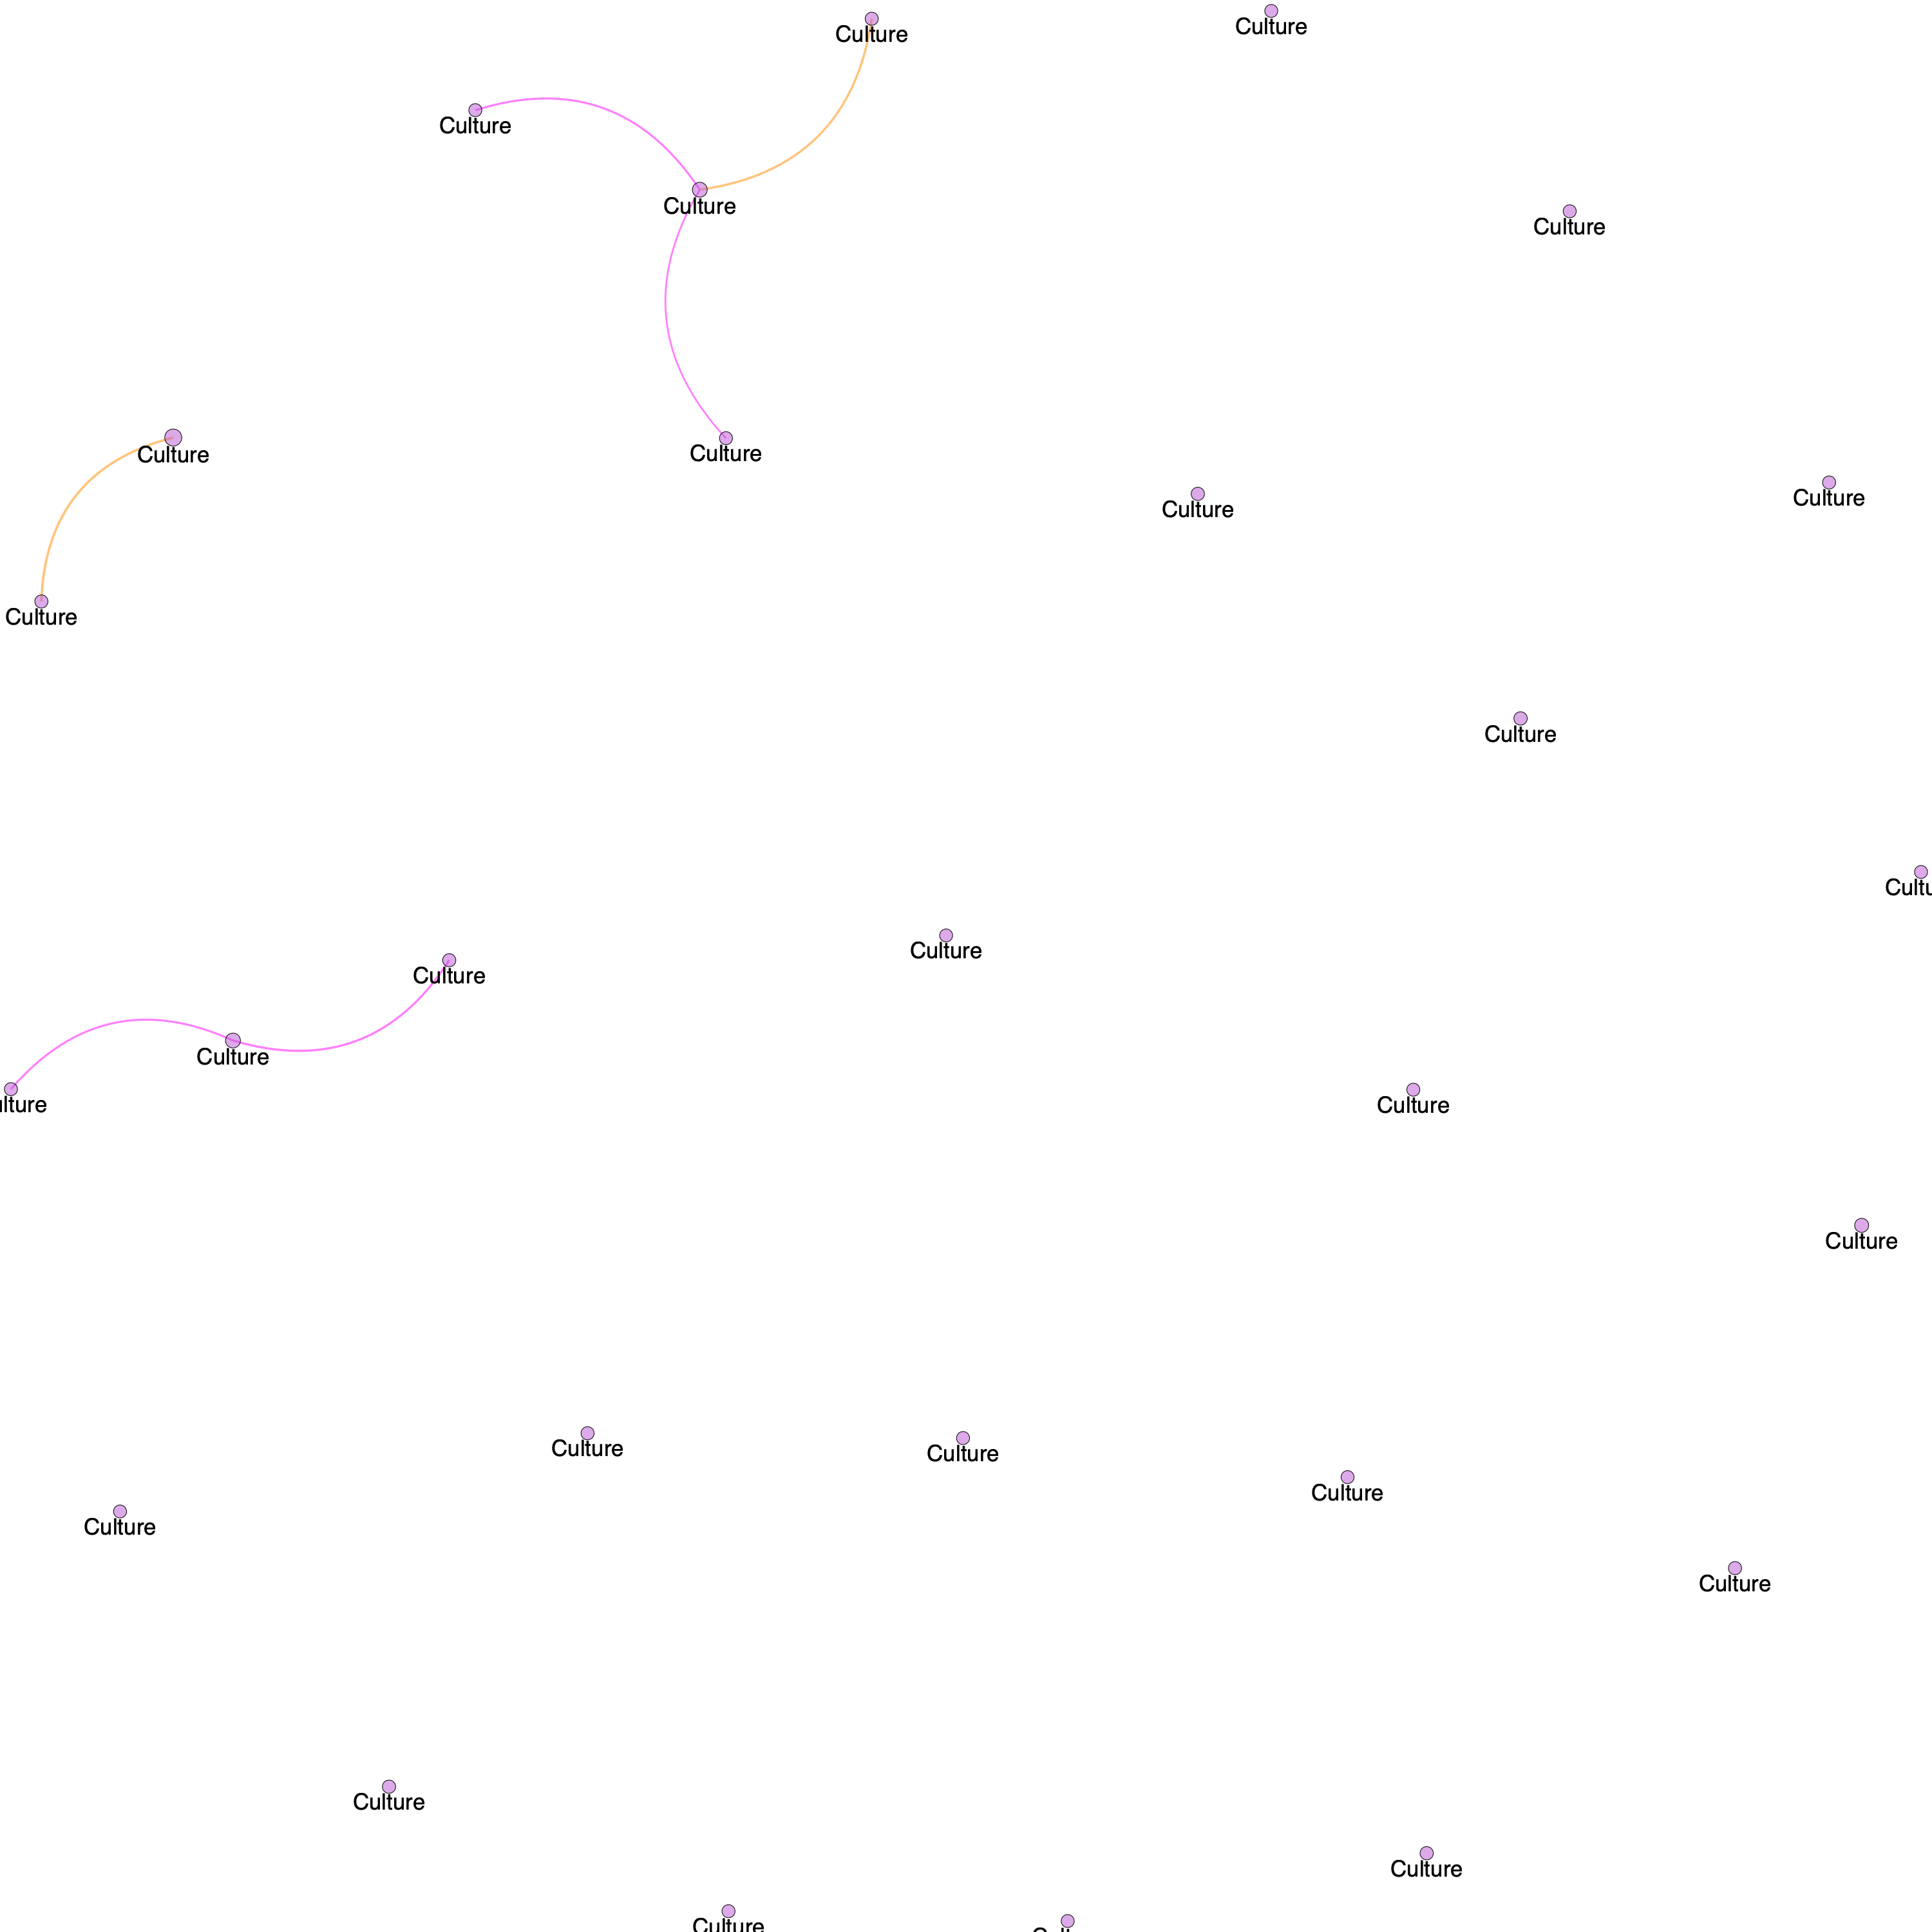
\includegraphics[width=0.32\linewidth]{figs/mysql_Mursuka_reduced_tagsub_cult.png}
\caption{Tagged scaffolds.}
\label{fig:scaftag}
\end{figure}

%\pgfplotstableread[col sep=comma]{Tag_ranking.csv}{\ranktable}
%\pgfplotstablegetcolsof{\loadedtable}
%\pgfmathtruncatemacro{\NoOfCols}{\pgfplotsretval-1}
%\begin{figure}[H]
%  \centering
%    \begin{tikzpicture}
%        \begin{axis}[
%        %height=5cm,width=8cm,
%        boxplot/draw direction = y,
%        x axis line style = {opacity=0},
%        axis x line* = bottom,
%        axis y line = left,
%        enlarge y limits,
%        ymin=0, ymax=150,
%        xtick=data,
%        xticklabels from table={\ranktable}{COUNT},
%        bar width=0.85/\NoOfCols,
%        cycle list={index of colormap=1 of Set1-8},
%        ymajorgrids,
%        xlabel = {k},
%        ylabel = {Degree CDF(k)},
%        ]
%        \foreach \i in {1,...,\NoOfCols} {
%            \addplot table [
%                x expr=\coordindex,
%                y index=\i,
%                col sep=comma,
%            ] {\ranktable};
%                \pgfplotstablegetcolumnnamebyindex{\i}\of{\ranktable}\to{\colname}
%                \addlegendentryexpanded{\colname};
%        }
%        \end{axis}
%    \end{tikzpicture}
%  \caption{Tag rankings.}
%  \label{fig:tagranks}
%\end{figure}

\subsection*{Markovian analysis}

\begin{figure}[H]
\centering
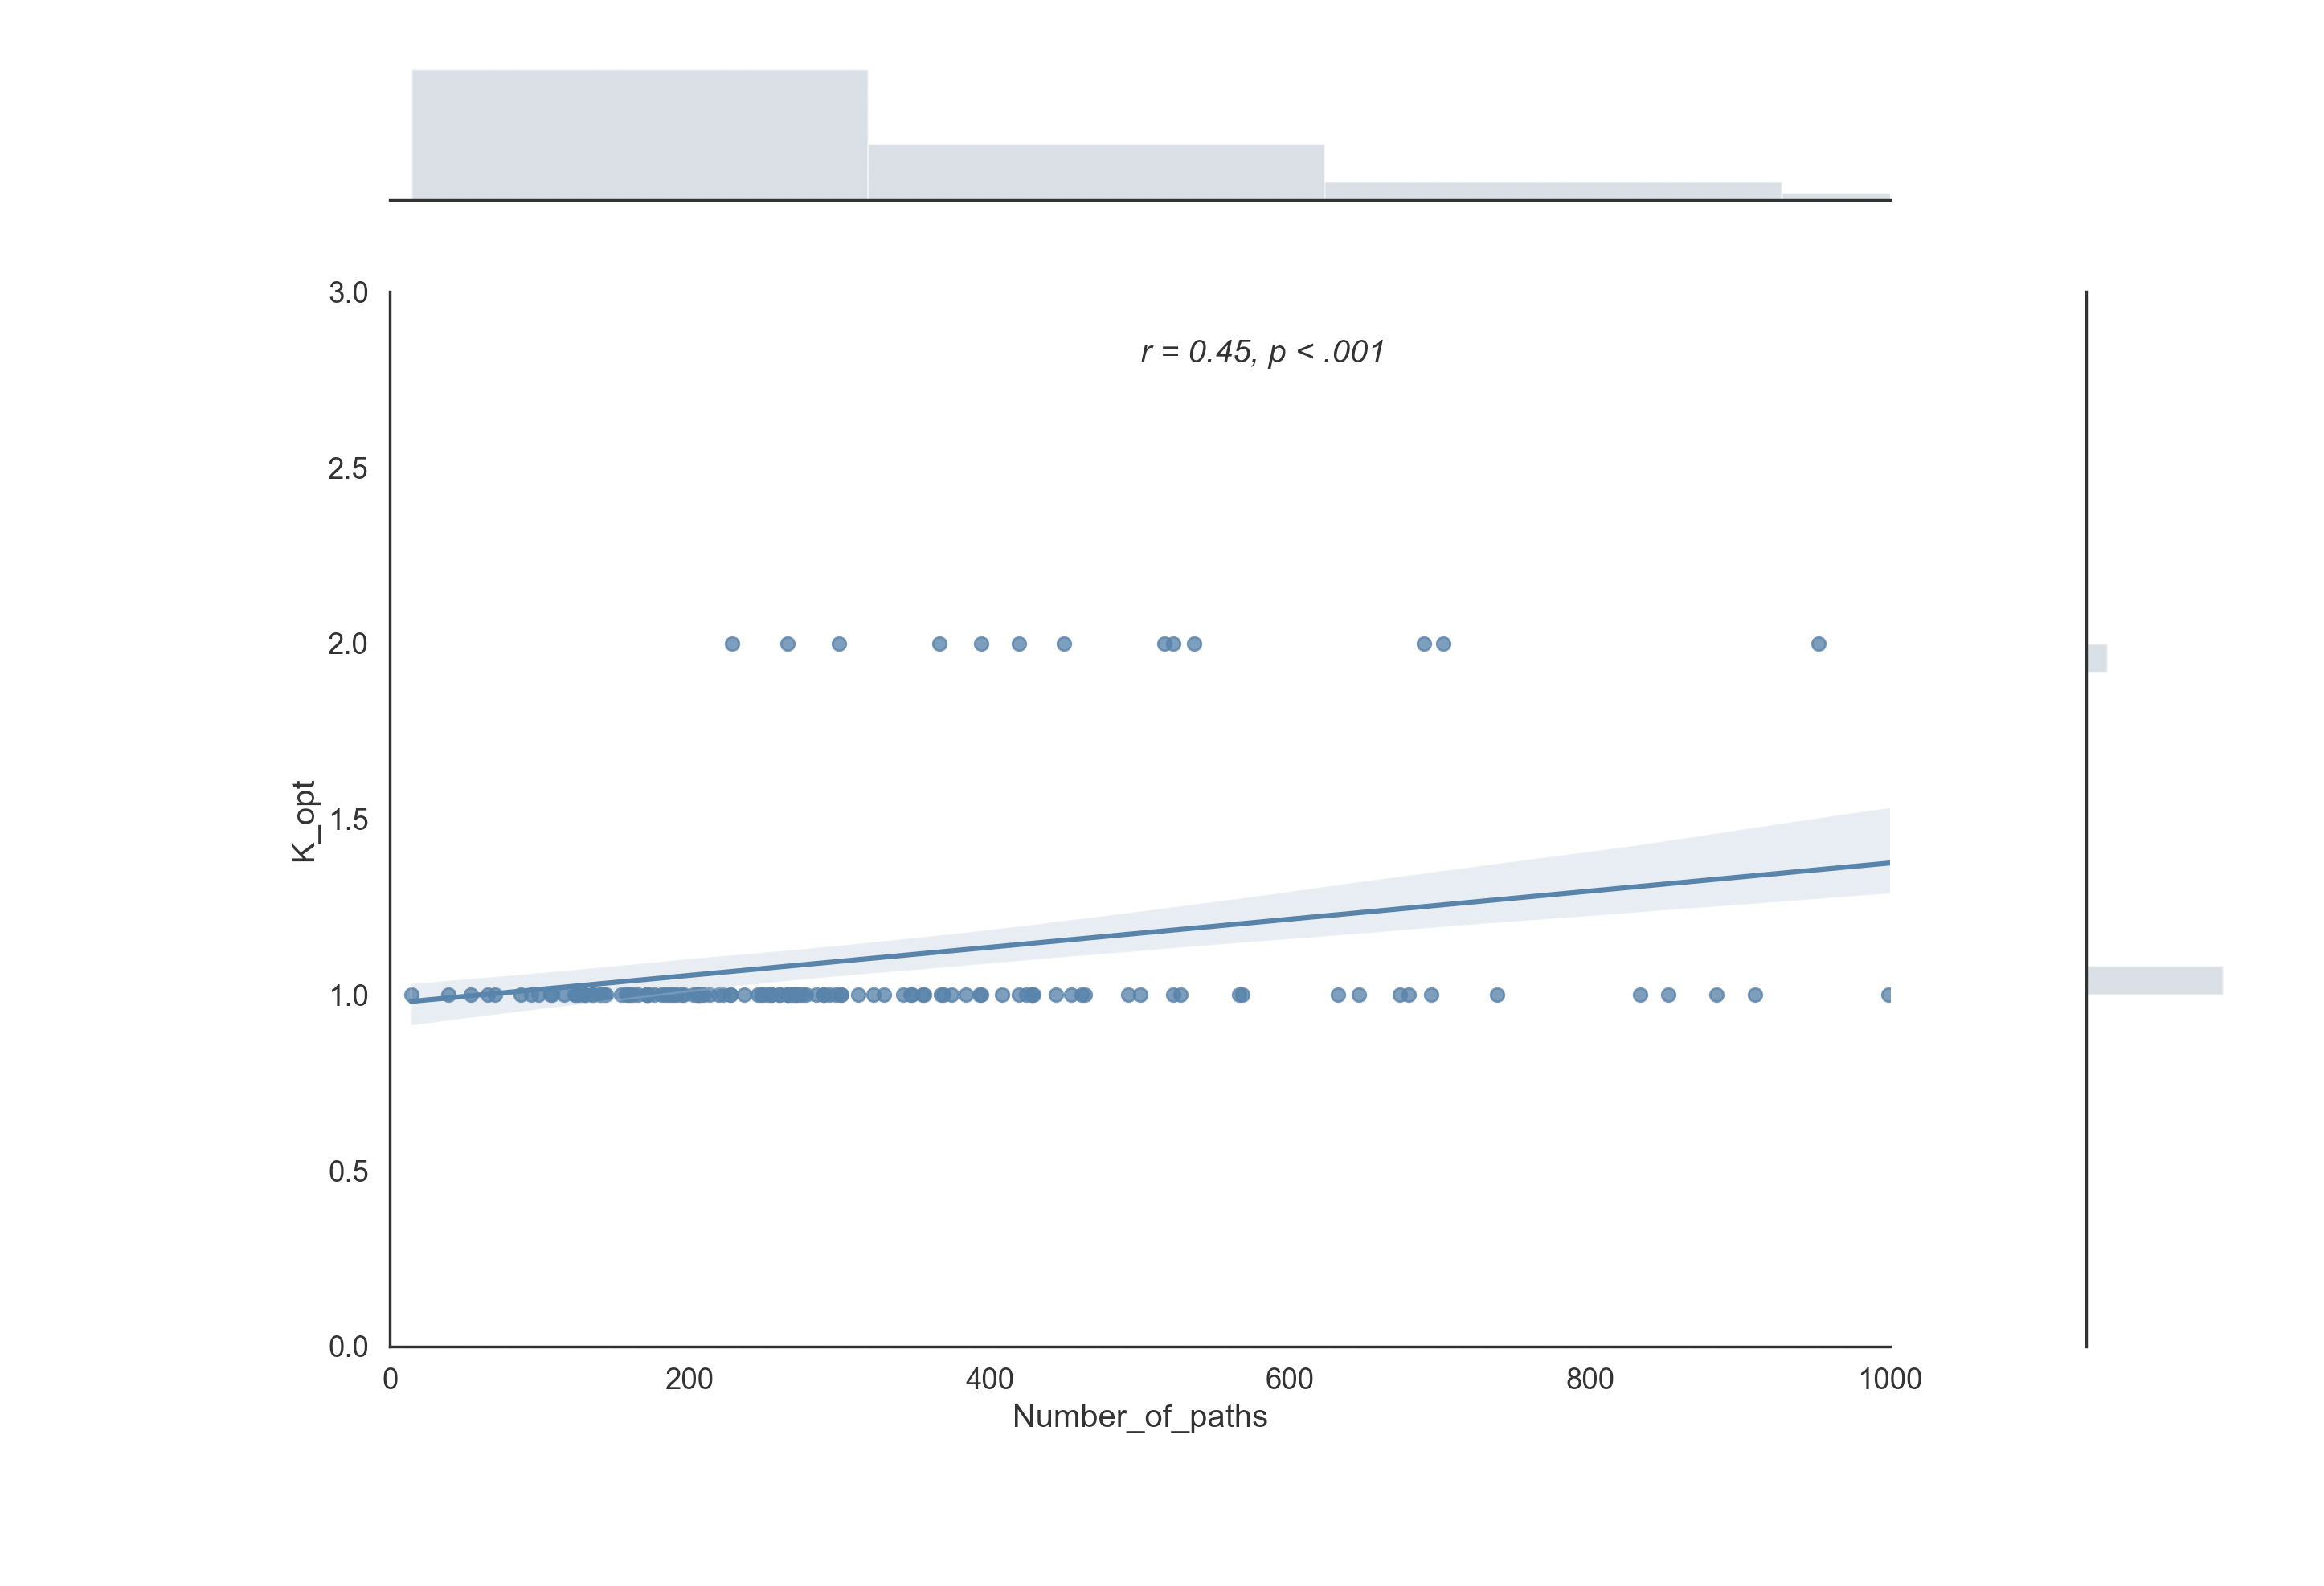
\includegraphics[width=0.5\linewidth]{figs/kopt.png}
\caption{This Fig supports that the proper description of user behaviour requires Markovian models of order two, although this result is quite weak due to the limited number of user paths, however still can be shown for some users... }
\label{fig:kopt}
\end{figure}

\subsection*{User statistics}

\begin{figure}[H]
\centering
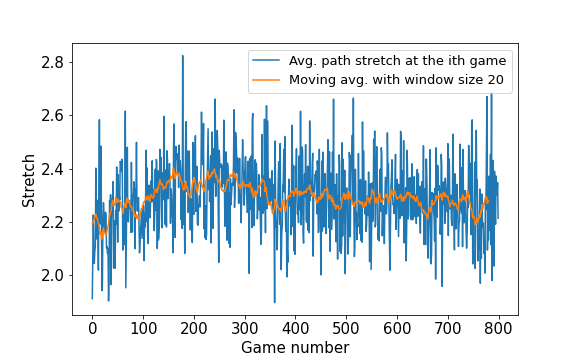
\includegraphics[width=0.45\linewidth]{figs/avg_stretch.png}
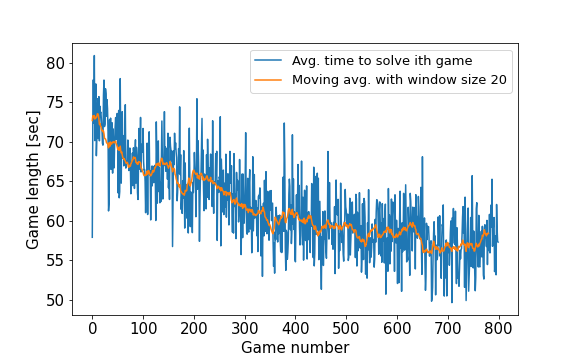
\includegraphics[width=0.45\linewidth]{figs/avg_game_length.png}
\caption{Average user statistics over 1000 games}
\label{fig:user_avg_stats}
\end{figure}

\subsection*{Subsection}

Example text under a subsection. Bulleted lists may be used where appropriate, e.g.

\begin{itemize}
\item First item
\item Second item
\end{itemize}

\subsubsection*{Third-level section}
 
Topical subheadings are allowed.

\section*{Discussion}

The Discussion should be succinct and must not contain subheadings.

\section*{Methods}

Topical subheadings are allowed. Authors must ensure that their Methods section includes adequate experimental and characterization data necessary for others in the field to reproduce their work.

\bibliography{sample}

\noindent LaTeX formats citations and references automatically using the bibliography records in your .bib file, which you can edit via the project menu. Use the cite command for an inline citation, e.g.  \cite{Hao:gidmaps:2014}.

For data citations of datasets uploaded to e.g. \emph{figshare}, please use the \verb|howpublished| option in the bib entry to specify the platform and the link, as in the \verb|Hao:gidmaps:2014| example in the sample bibliography file.

\section*{Acknowledgements (not compulsory)}

Acknowledgements should be brief, and should not include thanks to anonymous referees and editors, or effusive comments. Grant or contribution numbers may be acknowledged.

\section*{Author contributions statement}

Must include all authors, identified by initials, for example:
A.A. conceived the experiment(s),  A.A. and B.A. conducted the experiment(s), C.A. and D.A. analysed the results.  All authors reviewed the manuscript. 

\section*{Additional information}

To include, in this order: \textbf{Accession codes} (where applicable); \textbf{Competing interests} (mandatory statement). 

The corresponding author is responsible for submitting a \href{http://www.nature.com/srep/policies/index.html#competing}{competing interests statement} on behalf of all authors of the paper. This statement must be included in the submitted article file.

\begin{figure}[ht]
\centering
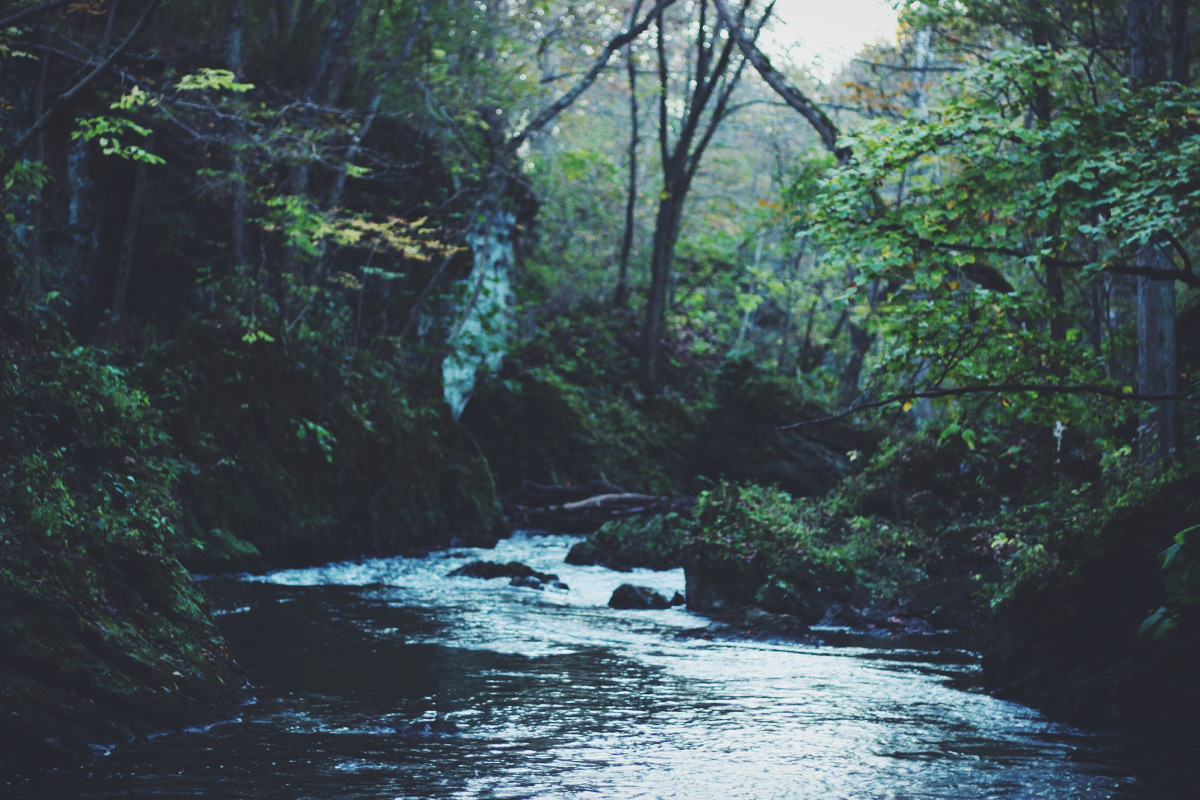
\includegraphics[width=\linewidth]{stream}
\caption{Legend (350 words max). Example legend text.}
\label{fig:stream}
\end{figure}

\begin{table}[ht]
\centering
\begin{tabular}{|l|l|l|}
\hline
Condition & n & p \\
\hline
A & 5 & 0.1 \\
\hline
B & 10 & 0.01 \\
\hline
\end{tabular}
\caption{\label{tab:example}Legend (350 words max). Example legend text.}
\end{table}

Figures and tables can be referenced in LaTeX using the ref command, e.g. Figure \ref{fig:stream} and Table \ref{tab:example}.

\end{document}